\documentclass{scrarticle}

\usepackage[utf8]{inputenc}
\usepackage[english]{babel}
\usepackage{csquotes}
\usepackage{float}

\usepackage{subcaption}
\DeclareCaptionFormat{custom}{\textbf{#1#2}\textit{\small #3}}
\captionsetup{format=custom}

\usepackage[backend=biber,natbib=true,sorting=none]{biblatex}
%\addbibresource{references.bib}
\addbibresource{../../references.bib}

\usepackage{graphicx}
%\graphicspath{ {./graphics/} }
\graphicspath{ {../../graphics/} }

\usepackage{hyperref}
\usepackage{amsfonts}       % blackboard math symbols
\usepackage{amsmath}

% Python pseudocode
\usepackage{pythonhighlight}
\lstdefinestyle{Py2}{numbers=left, style=mypython, frame=none}

\title{CLOOB: Modern Hopfield Networks with InfoLOOB Outperform CLIP}
\subtitle{Seminar in AI}

\author{%
  Pascal Pilz --- k12111234 \\
  \href{mailto:k12111234@students.jku.at}{k12111234@students.jku.at}}

% ==========================================================================================
% ==========================================================================================

\begin{document}

\maketitle

\section{Introduction}

The 2022 paper "CLOOB: Modern Hopfield Networks with InfoLOOB Outperform CLIP" by \citet{cloob} presents an improvement on CLIP (Contrastive Language-Image Pre-training, \citet{clip}), which is considered to be foundational and has been used as a benchmark several times \cite{cloob,foundational}.

Both methods use contrastive learning and aim to match text prompts with images in a zero-shot transfer learning setting, that is, performing predictions on classes that the model has not encountered during training. The main difference and improvement of CLOOB over CLIP is the use of modern Hopfield networks to overcome a problem of CLIP, namely the problem of "explaining away", which means that the model focuses on one object seen in the image while ignoring other important aspects \cite{cloob,explaining_away}. 

\citet{cloob} propose the integration of modern Hopfield networks into the model architecture of CLIP. They show that this, together with the use of a different objective function - InfoLOOB - leads to improved performance both in theory and in experimental setups.

\section{Background}

According to \citet{clip}, there has been a revolution in the field of natural language processing in the past decade. The development of "text-to-text" as a standardized input-output format combined with significant increases in compute power, model size, and data, has enabled the development of task-agnostic models that perform well on zero-shot transfer learning tasks.

\citet{clip} go on to explain that these developments suggested to them "that the aggregate supervision accessible to modern pre-training methods within web-scale collections of text surpasses that of high-quality crowd-labeled NLP datasets", prompting them to investigate whether scalable pre-trained methods learning directly from web text could achieve similar breakthroughs in computer vision.

\section{Multimodal Setting}

Both \citet{cloob,clip} project text prompts and images into the same latent space. The objective is to have the projected embeddings of positive text-image pairs close to each other while having negative pairs further apart in terms of their cosine similarity. This makes both methods multi-modal and contrastive in nature.

In both settings we have a set of $N$ iid drawn image-text pairs $\{(\mathbf{x}_1, \mathbf{y}_1), \dots, (\mathbf{x}_N, \mathbf{y}_N)\}$, where $(\mathbf{x}_1, \dots, \mathbf{x}_N)$ are the image embeddings obtained via a method such as a ResNet or a vision transformer model, and $(\mathbf{y}_1, \dots, \mathbf{y}_N)$ are the corresponding text encodings obtained via a continuous bag of words or a text transformer model \cite{cloob,clip}.

Both the image and text embeddings are normalized such that $\Vert \mathbf{x}_i \Vert = \Vert \mathbf{y}_j \Vert = 1$. Because of this, \citet{cloob} often talk of the uniformity of the sphere when discussing the distribution of the embeddings.

\section{CLIP and CLOOB}

\subsection{CLIP}

The basic architecture of CLIP can best be understood from Figure~\ref{fig:pseudo_clip}. During the training of CLIP, both an image encoder and a text encoder are trained in order to obtain the desired embedding properties. At inference time, the model predicts the most likely prompt from a given set of prompts that corresponds to a given image.

\begin{figure}[H]  % CLIP Pseudocode
  \begin{lstlisting}[style=Py2]
# image_encoder - ResNet or Vision Transformer
# text_encoder  - CBOW or Text Transformer
# I[n, h, w, c] - minibatch of aligned images
# T[n, l]       - minibatch of aligned texts
# W_i[d_i, d_e] - learned proj of image to embed
# W_t[d_t, d_e] - learned proj of text to embed
# t             - learned temperature parameter

# extract feature representations of each modality
I_f = image_encoder(I)  #[n, d_i]
T_f = text_encoder(T)   #[n, d_t]

# joint multimodal embedding [n, d_e]
I_e = l2_normalize(np.dot(I_f, W_i), axis=1)
T_e = l2_normalize(np.dot(T_f, W_t), axis=1)

# scaled pairwise cosine similarities [n, n]
logits = np.dot(I_e, T_e.T) * np.exp(t)

# symmetric loss function
labels = np.arange(n)
loss_i = cross_entropy_loss(logits, labels, axis=0)
loss_t = cross_entropy_loss(logits, labels, axis=1)
loss   = (loss_i + loss_t)/2
  \end{lstlisting}
  \caption{Numpy-like pseudocode for the core of an implementation of CLIP. Adapted from \citet{clip}}
  \label{fig:pseudo_clip}
\end{figure}

The training objective for CLIP is to minimize the InfoNCE loss function \eqref{eq:InfoNCE}.

\begin{equation}\label{eq:InfoNCE}
  \operatorname{L_{InfoNCE}} =
  - \frac{1}{N} \ln \sum_{i=1}^{N} \frac{\exp(\tau^{-1} \mathbf{x}_i^T \mathbf{y}_i)}{\sum_{j=1}^{N} \exp(\tau^{-1} \mathbf{x}_i^T \mathbf{y}_j)}
  - \frac{1}{N} \sum_{i=1}^{N} \ln \frac{\exp(\tau^{-1} \mathbf{x}_i^T \mathbf{y}_i)}{\sum_{j=1}^{N} \exp(\tau^{-1} \mathbf{x}_j^T \mathbf{y}_i)}
\end{equation}

\subsection{Modern Hopfield Networks}

A modern Hopfield network is a neural network that can store and retrieve patterns, making it a form of associative memory. During training, patterns are fed into the network and the weights are adjusted until an equilibrium is reached, and during inference a partial or noisy pattern can be fed in to obtain the stored pattern with the closest resemblance. This essentially creates archetypes, allowing the network to associate similar patterns and filter out noise.

The basic concept is best illustrated with an example from \citet{blogpost_cloob}, and the corresponding image in Figure~\ref{fig:tea_house}: For demonstration purposes, only the network features corresponding to a teacup, a teapot, a piece of cake, and a fork are arranged so that, when activated, they visually form the corresponding objects. In the rightmost images, we can see the underlying concept of a tea house, which is understood as the co-occurrence of a teacup, a teapot, a piece of cake, and a fork. This is what the network has stored in its weights. In the leftmost images, we have the objects observed in two different locations. This is the input to the network. We can see that all the objects corresponding to the stored concept of a tea house are present with varying levels of strength, but the modern Hopfield network is able to extract this information and, after performing a number of updates to network, the middle images can be observed.

\begin{figure}[H]
  \begin{center}
    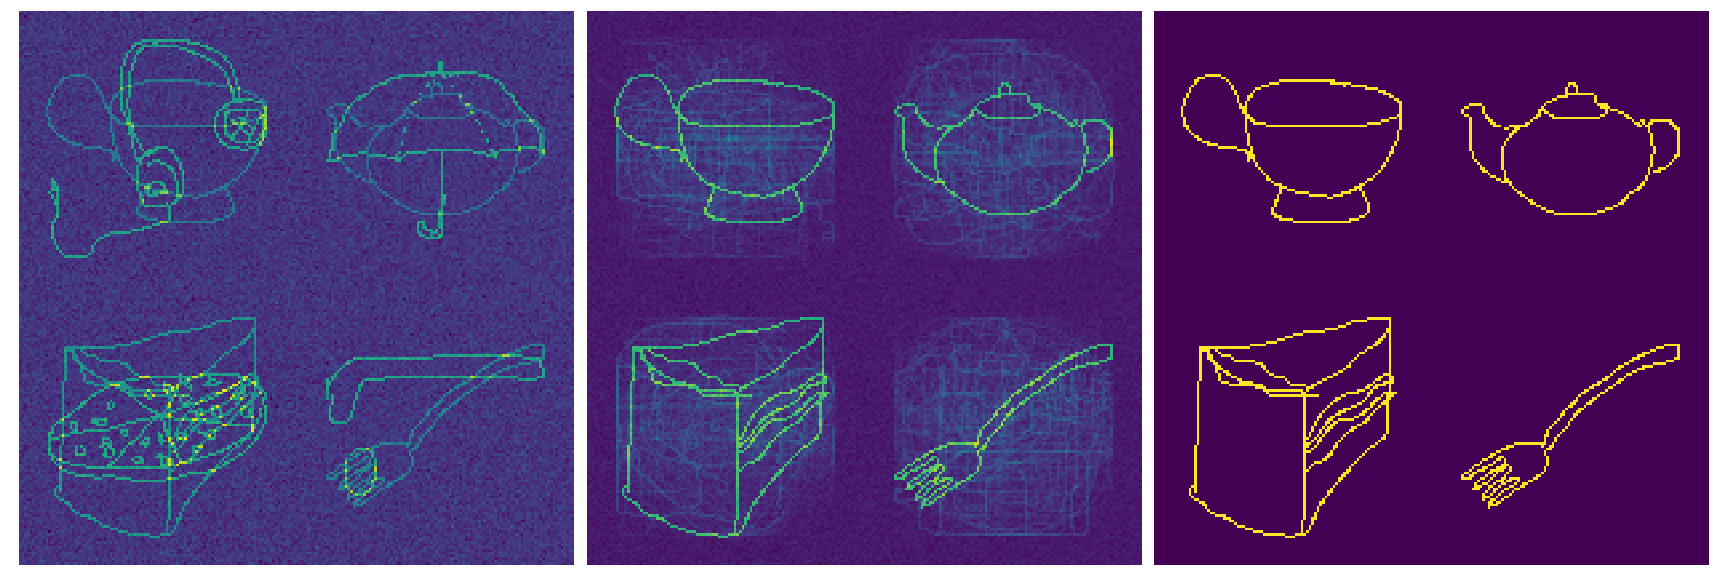
\includegraphics[width=\textwidth]{sketch_tea_hopfield}
    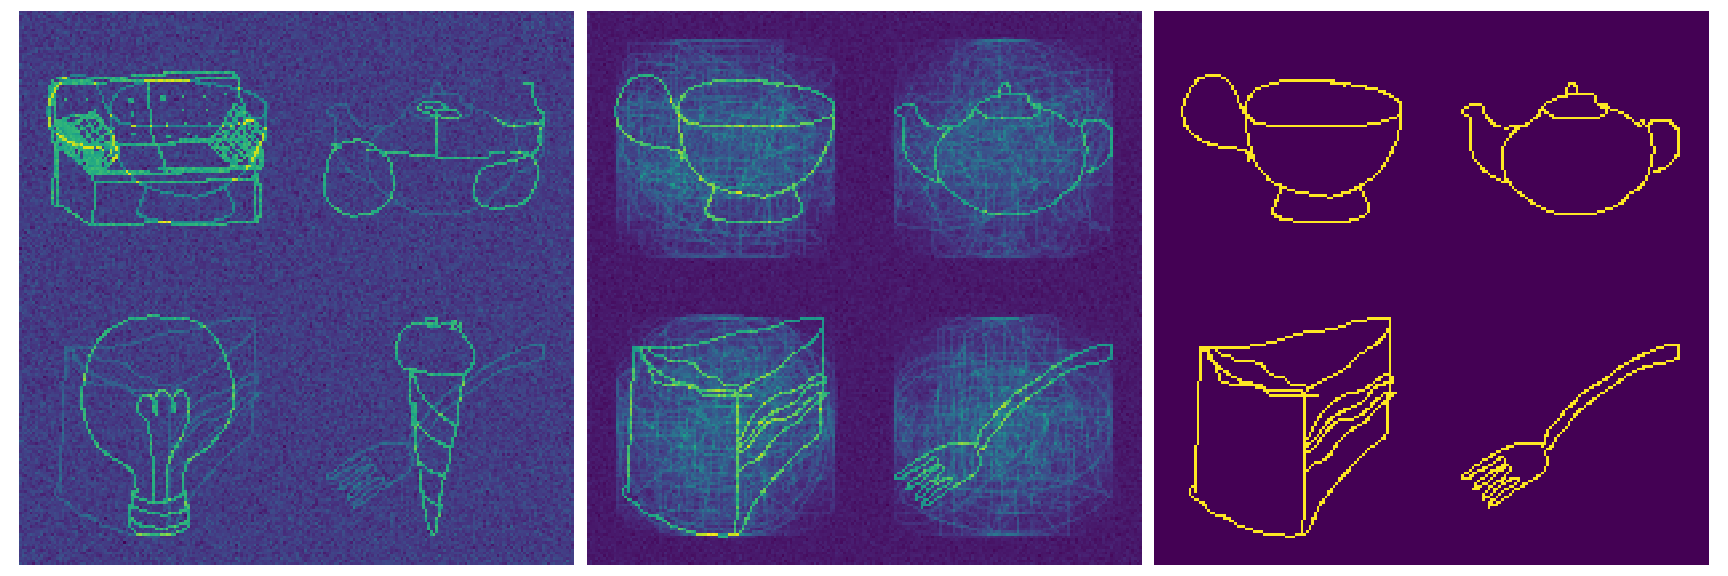
\includegraphics[width=\textwidth]{sketch_tea2_hopfield}
  \end{center}
  \caption{Stylized representation of the input and output to a Hopfield network that has the concept of a tea house stored in it. Adapted from \citet{blogpost_cloob}.}
  \label{fig:tea_house}
\end{figure}

Modern Hopfield networks can help with tackling the explaining away problem of CLIP, which is known in reasoning as the concept of accepting one cause of an event and dismissing all other causes \cite{explaining_away}. According to \citet{cloob}, this problem is caused by the model insufficiently extracting co-occurrences and covariance from the multimodal data. To combat this, \citet{cloob} suggest to use modern Hopfield networks to first store the calculated image and text embeddings and retrieve them immediately.

\subsection{CLOOB}

CLOOB's basic architecture is very similar to CLIP and can be seen in Figure~\ref{fig:pseudo_cloob}. During training, CLIP trains both an image encoder and a text encoder in order to obtain the desired embedding properties. At inference time, the model predicts the most likely prompt from a given set of prompts that corresponds to a given image.

\begin{figure}[H]  % CLOOB Pseudocode
  \begin{lstlisting}[style=Py2]
# image_encoder       - ResNet or Vision Transformer
# text_encoder        - CBOW or Text Transformer
# I [n , h , w , c ]  - minibatch of aligned images
# T [n , l ]          - minibatch of aligned texts
# W_i [ d_i , d_e ]   - learned proj of image to embed
# W_t [ d_t , d_e ]   - learned proj of text to embed
# b                   - inverse temperature Hopfield retrieval
# t                   - learned temperature parameter

# extract feature representations of each modality
I_f = image_encoder(I)  #[n, d_i]
T_f = text_encoder(T)   #[n, d_t]

# joint multimodal embedding
x = l2_normalize(I_f @ W_i)   #[n, d_e]
y = l2_normalize(T_f @ W_t)   #[n, d_e]

# Hopfield retrieval H with batch stored
# H(beta, A, B) = B.T @ softmax(beta * A @ B.T)
U_x = H(b, x, x).T #[n, d_e]
U_y = H(b, y, x).T #[n, d_e]
V_x = H(b, x, y).T #[n, d_e]
V_y = H(b, y, y).T #[n, d_e]

# normalize retrievals
U_x = l2_normalize(U_x)   #[n, d_e] 
U_y = l2_normalize(U_y)   #[n, d_e] 
V_x = l2_normalize(V_x)   #[n, d_e] 
V_y = l2_normalize(V_y)   #[n, d_e]

# loss: info_loob(tau, anchors, samples) 
loss_i = info_loob(t, U_x, U_y)
loss_t = info_loob(t, V_y, V_x)
loss = (loss_i + loss_t) * t
  \end{lstlisting}
  \caption{Numpy-like pseudocode for the core of an implementation of CLOOB. Adapted from \citet{cloob}}
  \label{fig:pseudo_cloob}
\end{figure}

The training objective for CLOOB is to minimize the InfoLOOB loss function \eqref{eq:InfoLOOB}.

\begin{equation}\label{eq:InfoLOOB}
  \operatorname{L_{InfoLOOB}} =
  -\frac{1}{N} \ln \sum_{i=1}^{N} \frac{\exp(\tau^{-1}\mathbf{x}_i^T \mathbf{y}_i)}{\sum_{j \neq i}^{N} \exp(\tau^{-1} \mathbf{x}_i^T \mathbf{y}_j)}
  - \frac{1}{N} \sum_{i=1}^{N} \ln \frac{\exp(\tau^{-1}\mathbf{x}_i^T \mathbf{y}_i)}{\sum_{j\neq i}^{N}\exp(\tau^{-1} \mathbf{x}_j^T \mathbf{y}_i)}
\end{equation}

\subsection{InfoLOOB and the Saturation Effect}

To explain the saturation effect, it is useful to consider only the second sum and the first sample of the InfoNCE \eqref{eq:InfoNCE} and InfoLOOB objective~\ref{eq:InfoLOOB}:

\begin{align}
\operatorname{L_{InfoNCE}}(\mathbf{y}_1)
&= -\ln\frac{\overbrace{\exp(\tau^{-1} \mathbf{x}_1^T \mathbf{y}_1)}^{a}}{\underbrace{\exp(\tau^{-1}\mathbf{x}_1^T \mathbf{y}_1)}_{a} + \underbrace{\textstyle\sum_{j=2}^{N} \exp(\tau^{-1} \mathbf{x}_j^T \mathbf{y}_ 1)}_{b}} \\
\operatorname{L_{InfoLOOB}}(\mathbf{y}_1)
&= -\ln\frac{\overbrace{\exp(\tau^{-1} \mathbf{x}_1^T \mathbf{y}_1)}^{a}}{\underbrace{\textstyle\sum_{j=2}^{N} \exp(\tau^{-1} \mathbf{x}_j^T \mathbf{y}_ 1)}_{b}}
\end{align}

Inherently, minimizing the InfoNCE loss is equivalent to increasing $a$, the similarity of the positive pair, and decreasing $b$, the similarity of the negative pairs. The denominator includes both $a$ and $b$, which means that if $a$ is large relative to $b$, the value of the fraction will change little with any change in $a$ or $b$.

\citet{cloob} call this the saturation effect, and according to them, it is a problem when using modern Hopfield networks, since the retrieved embeddings naturally have a higher similarity to each other. To combat the saturation effect, they suggest using the InfoLOOB objective, which excludes the positive pair $a$ from the denominator.

\section{Experiments}

\citet{cloob} conducted a series of experiments to compare CLOOB with CLIP, pre-training once on the Conceptual Caption (CC) dataset and once on the Yahoo Flickr Creative Commons (YFCC) dataset. They also conducted ablation studies to determine the effects of two newly introduced changes, (1) modern Hopfield networks and (2) InfoLOOB.

For each of the three experiments, CLOOB was implemented based on OpenCLIP by \citet{open_clip}. Similarly, CLIP was reimplemented based on OpenCLIP. OpenCLIP achieves equivalent results to those reported by \citet{clip}.

\subsection{Zero-Shot Transfer Learning}

\subsubsection{Conceptual Caption}

The Conceptual Captions (CC) dataset \cite{cc} consists of 2.9 million images with high-quality, detailed text descriptions. Since the original CLIP was not trained on this dataset, the authors of CLOOB used their own reimplementation for the comparison. For both models they used a ResNet-50 and a BERT architecture to encode the image-text pairs. The results of zero-shot transfer learning experiments on seven different datasets are shown in Table~\ref{table:cc}.

\begin{table}[H]
    \begin{center}
        \begin{tabular}{l | c c | c c | c c }
Dataset       &CLIP RN-50     &CLOOB RN-50                &CLIP RN-50               &CLOOB RN-50    \\
\hline
Birdsnap      &$2.26\pm0.20$  &$\mathbf{3.06\pm0.30}$     &$2.8\pm0.16$     &$\mathbf{3.24\pm0.31}$ \\
Country211    &$0.67\pm0.11$  &$0.67\pm0.05$              &$0.7\pm0.04$     &$0.73\pm0.05$          \\
Flowers102    &$12.56\pm0.38$ &$13.45\pm1.19$             &$13.32\pm0.43$   &$14.36\pm1.17$         \\
GTSRB         &$7.66\pm1.07$  &$6.38\pm2.11$              &$8.96\pm1.70$    &$7.03\pm1.22$          \\
UCF101        &$20.98\pm1.55$ &$22.26\pm0.72$             &$21.63\pm0.65$   &$\mathbf{23.03\pm0.85}$\\
Stanford Cars &$0.91\pm0.10$  &$\mathbf{1.23\pm0.10}$     &$0.99\pm0.16$    &$\mathbf{1.41\pm0.32}$ \\
ImageNet      &$20.33\pm0.28$ &$\mathbf{23.97\pm0.15}$    &$21.3\pm0.42$    &$\mathbf{25.67\pm0.22}$\\
ImageNet V2   &$20.24\pm0.50$ &$\mathbf{23.59\pm0.15}$    &$21.24\pm0.22$   &$\mathbf{25.49\pm0.11}$\\
        \end{tabular}
    \end{center}
    \caption{Zero-shot results for models trained on CC with ResNet-50 vision encoders for two different checkpoints. Results are given as mean accuracy over 5 runs. Statistically significant results are shown in bold. CLIP and CLOOB were trained for 31 epochs while CLIP* and CLOOB* were trained for 128 epochs. Adapted from \citet{cloob}.}
    \label{table:cc}
\end{table}

\subsubsection{Yahoo Flickr Creative Commons}

The Yahoo Flickr Creative Commons 100 Million (YFCC100M) dataset \cite{yfcc} consists of 99.2 million images, of which the authors chose a subset of 15 million images with less rich textual description then the CC dataset. Again, since the original CLIP was not trained on this dataset, the authors of CLOOB used their own reimplementation for the comparison. For both models they used a ResNet-50, a ResNet-101, and a ResNet-50x4, as well as a BERT architecture to encode the image-text pairs. The results of zero-shot transfer learning experiments on seven different
datasets are shown in Table~\ref{table:yfcc}

\begin{table}[H]
    \begin{center}
        \begin{tabular}{l | c c | c c | c c }
&\multicolumn{2}{|c|}{RN-50}    &\multicolumn{2}{|c|}{RN-101}   &\multicolumn{2}{|c}{RN-50x4}  \\
Dataset         &CLIP   &CLOOB  &CLIP   &CLOOB  &CLIP   &CLOOB  \\
\hline
Birdsnap        &$21.8$             &$\mathbf{28.9}$    &$22.6$ &$\mathbf{30.3}$    &$20.8$ &$\mathbf{32.0}$    \\
Country211      &$6.9$              &$\mathbf{7.9}$     &$7.8$  &$\mathbf{8.5}$     &$8.1$  &$\mathbf{9.3}$     \\
Flowers102      &$48.0$             &$\mathbf{55.1}$    &$48.0$ &$\mathbf{55.3}$    &$50.1$ &$\mathbf{54.3}$    \\
GTSRB           &$7.9$              &$\mathbf{8.1}$     &$7.4$  &$\mathbf{11.6}$    &$9.4$  &$\mathbf{11.8}$    \\
UCF101          &$\mathbf{27.2}$    &$25.3$             &$28.6$ &$\mathbf{28.8}$    &$31.0$ &$\mathbf{31.9}$    \\
Stanford Cars   &$3.7$              &$\mathbf{4.1}$     &$3.8$  &$\mathbf{5.5}$     &$3.5$  &$\mathbf{6.1}$     \\
ImageNet        &$34.6$             &$\mathbf{35.7}$    &$35.3$ &$\mathbf{37.1}$    &$37.7$ &$\mathbf{39.0}$    \\
ImageNet V2     &$33.4$             &$\mathbf{34.6}$    &$34.1$ &$\mathbf{35.6}$    &$35.9$ &$\mathbf{37.3}$    \\
        \end{tabular}
    \end{center}
    \caption{Zero-shot results for the CLIP reimplementation and CLOOB using different ResNet architectures trained on YFCC. Adapted from \citet{cloob}.}
    \label{table:yfcc}
\end{table}

\subsection{Ablation studies}

\citet{cloob} found that the interplay of modern Hopfield networks with InfoLOOB is crucial, as either one alone shows little to no improvement (see Table~\ref{table:ablation_scores}).

\begin{table}[H]
  \begin{center}
    \scalebox{0.7}{
      \begin{tabular}{l | cccc | cccc}
                &         &         &InfoNCE  &nfoLOOB  &         &           &InfoNCE    &InfoLOOB \\
Dataset         &InfoNCE  &InfoLOOB &Hopfield &Hopfield &InfoNCE* &InfoLOOB*  &Hopfield*  &Hopfield*  \\
\hline
Birdsnap        &$\mathbf{2.58}$  &$2.37$ &$1.67$ &$2.53$ &$2.15$ &$1.89$ &$2.15$ &$\mathbf{3.39}$ \\
Country211      &$0.53$ &$0.63$ &$0.54$ &$\mathbf{0.76}$ &$0.62$ &$0.62$ &$0.66$ &$\mathbf{0.79}$ \\
Flowers102      &$13.16$ &$13.03$ &$11.53$ &$\mathbf{14.24}$ &$11.79$ &$11.57$ &$10.86$ &$\mathbf{14.24}$  \\
GTSRB           &$4.47$ &$4.39$ &$5.76$ &$\mathbf{5.86}$ &$\mathbf{9.25}$ &$6.93$ &$6.24$ &$8.67$ \\
UCF101          &$\mathbf{23.68}$ &$19.14$  &$20.56$  &$22.29$  &$21.33$  &$20.56$  &$21.40$  &$\mathbf{24.05}$\\
Stanford Cars   &$\mathbf{1.38}$  &$1.33$ &$1.24$ &$1.37$ &$1.26$ &$1.19$ &$1.24$ &$\mathbf{1.62}$ \\
ImageNet        &$21.74$  &$22.13$  &$19.04$  &$\mathbf{24.21}$ &$22.80$  &$22.69$  &$20.69$  &$\mathbf{25.59}$ \\
ImageNet V2     &$21.45$  &$21.65$  &$18.97$  &$\mathbf{23.80}$ &$22.44$  &$22.13$  &$20.22$  &$\mathbf{25.50}$
      \end{tabular}
    }
  \end{center}
  \caption{Influence of loss functions and Hopfield retrieval for models pre-trained on CC for 31 epochs (left) and 128 epochs (right, indicated by *). Adapted from \citet{cloob}.}
  \label{table:ablation_scores}
\end{table}

They claim that this is due to the underfitting tendency of modern Hopfield networks counteracting the overfitting tendency of the InfoLOOB objective. To support this claim they show a comparison of the cosine similarity of matched and unmatched pairs. Figure~\ref{fig:ablation_density} shows that modern Hopfield networks lead to higher similarity between unmatched and matched pairs, while InfoLOOB leads to higher similarity in matched pairs.

\begin{figure}[H]
  \begin{center}
    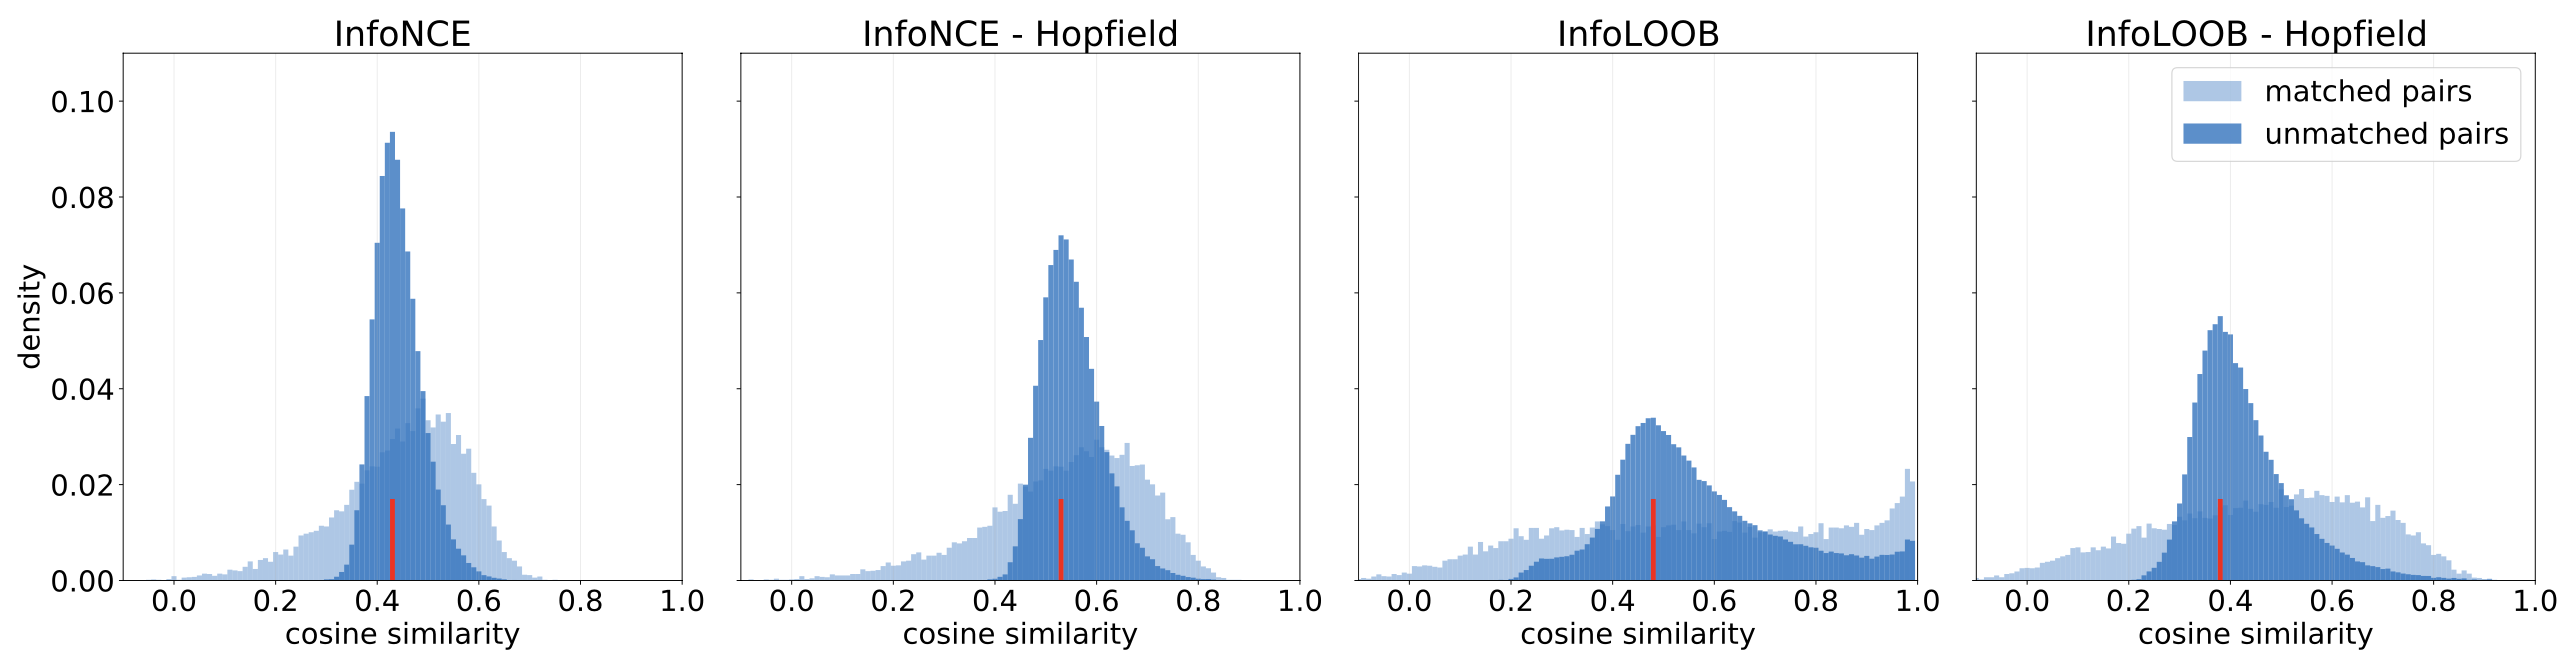
\includegraphics[width=\textwidth]{ablation}
  \end{center}
  \caption{Distribution of the cosine similarity of matched pairs and the cosine similarity of the 10 unmatched pairs that have the highest similarity score with the anchor. Adapted from \citet{cloob}.}
  \label{fig:ablation_density}
\end{figure}

In addition, \citet{cloob} discuss the ability of modern Hopfield networks to extract more covariance structure during learning. This can be seen in Figure~\ref{fig:eigenvalues}, which shows the number of eigenvalues needed to reconstruct 99\% of the covariance matrix of the corresponding embeddings at an early point in training compared to a later point in training. A higher number indicates that the covariance matrix is more complex.

\begin{figure}[H]
  \begin{center}
    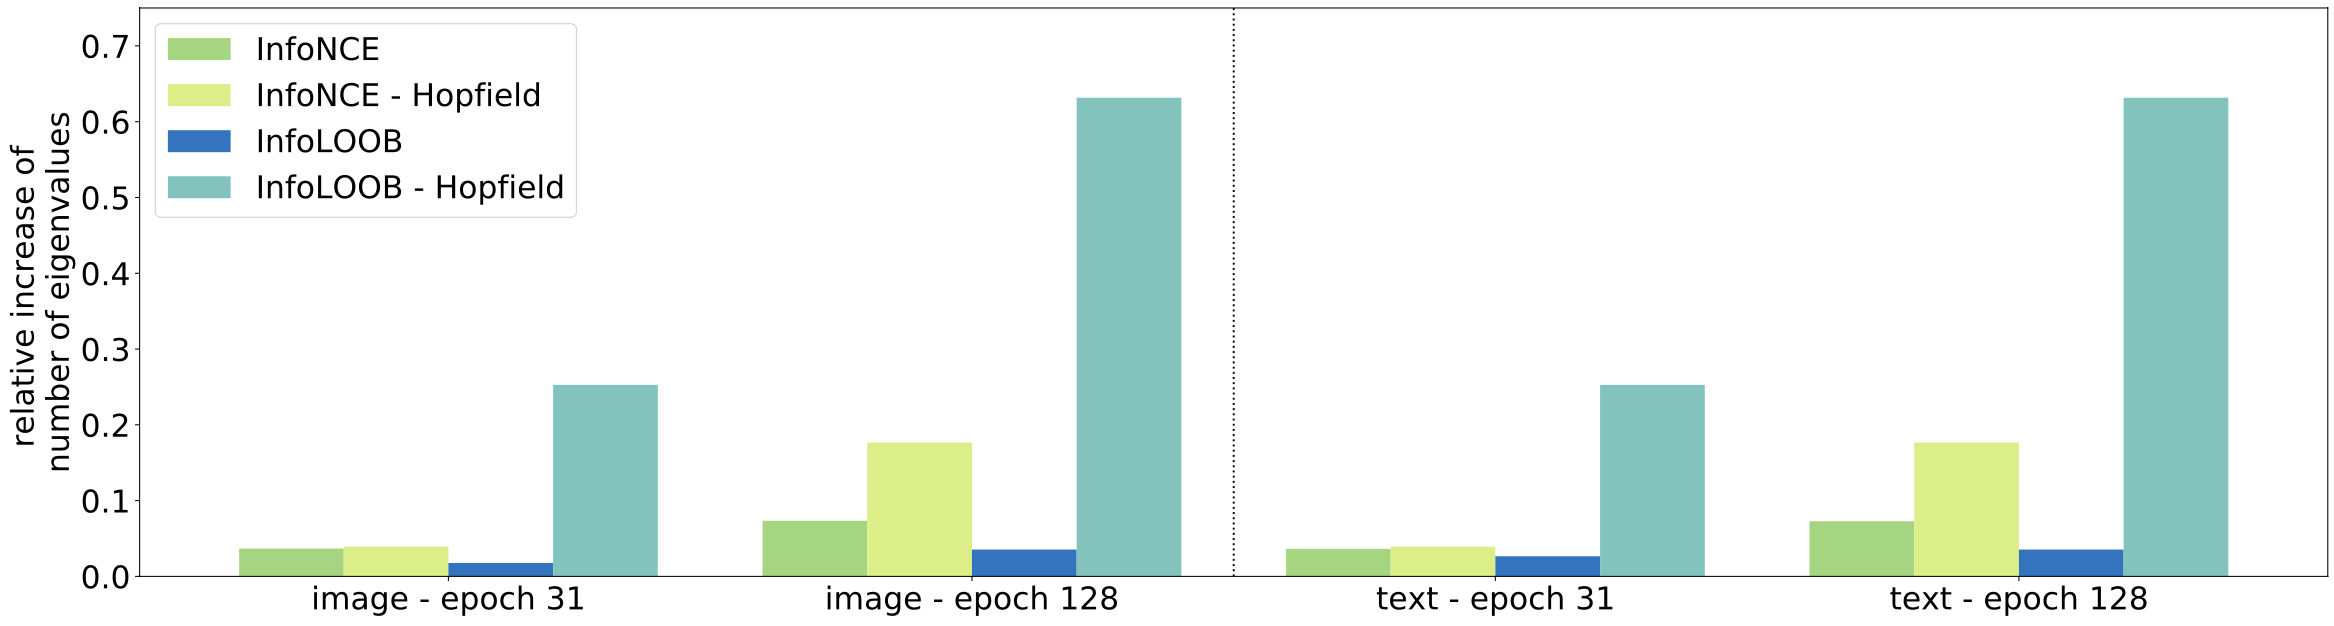
\includegraphics[width=\textwidth]{eigenvalues}
  \end{center}
  \caption{Relative change in the number of the effective eigenvalues of the embedding covariance matrices, which were obtained from image and text encoders at two different training points. Adapted from \citet{cloob}.}
  \label{fig:eigenvalues}
\end{figure}

\section{Discussion and Critical Assessment}

Unlike Table~\ref{table:cc} (Table 1 in \citet{cloob}) and the corresponding experiment, \citet{cloob} do not explicitly explain the meaning of the bold-highlighted text in Table~\ref{table:yfcc} (Table 3 in \citet{cloob}) and whether or not multiple tests were performed and the results averaged. Therefore, it is not clear to me how the YFCC experiment was performed and what the highlighting in Table~\ref{table:yfcc} is supposed to show. The same problem exists with Table~\ref{table:ablation_scores} (Table A1 in \citet{cloob}). \citet{cloob} do not explicitly discuss aspects such as data and energy efficiency when it comes to CLOOB. Nor do they discuss possible reasons for not using modern Hopfield networks.

The aspects of modern Hopfield networks concerning their covariance structure were difficult for me to understand. Nevertheless, it should be noted that \citet{cloob} take great care to explain concepts in an understandable and detailed way, making it easier to understand for readers with less experience in the field. Furthermore, they fulfil all relevant points of the "NeurIPS 2022 Paper Checklist Guidelines". In addition, they strive to include as many potentially interesting theoretical and experimental results as possible in the appendix.

% ==========================================================================================
\clearpage
\printbibliography

\end{document}